\documentclass[a4paper]{article}
% Uncomment the following line to allow the usage of graphics (.png, .jpg)
\usepackage[pdftex]{graphicx}
% Allow the usage of utf8 characters
\usepackage[utf8]{inputenc}
\usepackage{enumerate}
\usepackage{amssymb}
\usepackage{icomma}
\usepackage{xcolor}
\usepackage{colortbl}
\usepackage{siunitx}
\sisetup{locale=DE} 
\usepackage{tikz}
\usepackage{href-ul}
\hypersetup{
	colorlinks=true,
	linkcolor=blue,
	urlcolor=blue}
\usepackage{geometry}
\geometry{a4paper, top=15mm, left=15mm, right=15mm, bottom=15mm,
	headsep=10mm, footskip=12mm}

\begin{document}
	
	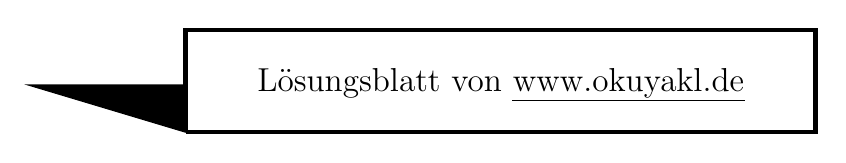
\begin{tikzpicture}(10,3)
		\draw[ultra thick](2,0) --(10,0) -- (10,1.3) --(2,1.3) -- (2,0);
		\draw[fill=black](2,0)-- (0,.6) -- (2,.6) -- (2,0);
		\node at (6,.6) {\large Lösungsblatt von \href{https://www.okuyakl.de}{www.okuyakl.de}};
	\end{tikzpicture}
	
{\bf Elementare Brüche als Kommazahl, Prozent und Kreisdiagramm}

\begin{enumerate}[1.]
{\bf \item Endliche Dezimalbrüche}

\renewcommand{\arraystretch}{4}
\begin{tabular}{|>{\columncolor[gray]{.8}}p{1.5 cm}|p{4.84 cm}|p{4.84 cm}|p{4.84 cm}|}
	\hline
	\rowcolor[gray]{.8} Bruch & Erweitert auf Stufenzahl & Dezimalbruch & Prozent \% \\
	\hline
	${1 \over 2}$& ${5\over 10}$ & $0,5$ & $50 ~\% $  \\
	\hline
	${1 \over 4}$&${25 \over 100}$ & $0,25$ & $25 ~\% $ \\
	\hline
	${1 \over 5}$&${2 \over 10}$  & $0,2$ & $20 ~\% $ \\
	\hline
	${1 \over 8}$&${125 \over 100}$  & $0,125$ & $12,5 ~\% $ \\
	\hline
	${1 \over 10}$&${1 \over 10}$  & $0,1$ & $10 ~\% $ \\
	\hline
\end{tabular}

{\bf \item Unendliche Dezimalbrüche}

\renewcommand{\arraystretch}{4}
\begin{tabular}{|>{\columncolor[gray]{.8}}p{1.5 cm}|p{7.5 cm}|p{7.5 cm}|}
	\hline
	\rowcolor[gray]{.8} Bruch & Periodischer Dezimalbruch & Prozent ~\% \\
	\hline
	${1 \over 3}$& $0,\overline{3}$ & $33,\overline{3} ~\% $ \\
	\hline
	${1 \over 6}$& $0,1\overline{6}$ & $16,\overline{6} ~\% $\\
	\hline
	${1 \over 7}$& $0,\overline{142857}$ & $14,2857\overline{142857} ~\% $\\
	\hline
	${1 \over 9}$& $0,\overline{1}$ & $11,\overline{1} ~\% $\\
	\hline
\end{tabular}

\newpage
{\bf \item Stelle alle Brüche jeweils als Kreisdiagramm dar!}

\includegraphics[width=16 cm]{kreidi120}
\end{enumerate} 


\begin{center}
	\includegraphics[width=7 cm]{../../viecher/endcomic.pdf}
	
	Hier geht es zurück zum \href{https://www.okuyakl.de/math/m6bkpL120/aa120.pdf}{Aufgabenblatt}
\end{center}
\end{document}
\end{document}

